\documentclass[10pt,        % Don't change the font size!
               a4paper,     % Don't change the paper size!
               journal,     % Journal paper format
%               draft       % Enable this parameter to get a draft version.
               ]{IEEEtran}
\makeatletter

\def\markboth#1#2{\def\leftmark{\@IEEEcompsoconly{\sffamily}\MakeUppercase{\protect#1}}%
\def\rightmark{\@IEEEcompsoconly{\sffamily}\MakeUppercase{\protect#2}}}
\makeatother

% Packages
%\usepackage[latin1]{inputenc}
\usepackage[utf8]{inputenc}
\usepackage[T1]{fontenc}
\usepackage{xcolor}
\usepackage{graphicx}
\usepackage{subcaption}

% \graphicspath{{../pdf/}{../jpeg/}}
% \DeclareGraphicsExtensions{.pdf,.jpeg,.png}

\begin{document}

% paper title
\title{Neural Architecture Search and tinyML: A Survey}
\author{Daniel~Duclos-Cavalcanti}

% The paper headers
\markboth{Seminar for VLSI Entwurfsverfahren, Summer Term 2022}%
{Daniel Duclos-Cavalcanti: Network Architecture Search (NAS)}

% make the title area
\maketitle

%\thanks{Daniel D-C. is with the Department
%of Electrical and Computer Engineering, Technical University of Munich, Bavaria, DE.}% <-this % stops a space

\begin{abstract}
There is no denying the increasing success that Deep Neural Networks (DNNs)
have displayed across various tasks such as image classification, speech recognition, machine translation
and many others. This progress can be attributed largely due to \textit{architecture engineering},
which is a process that requires immense domain expertise, intuition and some amount of trial
and error. This is not ideal as it is both time consuming and error-prone. Neural Architecture Search (NAS)
rises as the next logical step aiming to both automate architecture discovery and further the understanding
of the inner workings of DNNs. This field has grown remarkably within the last 5 years and among the many challenges
of NAS, there are concerns regarding computational costs and time feasability. This however changes within the context
of \textit{tinyML}, which is an expanding field at the intersection of machine learning and embedded systems.
Due to the resource constrained conditions involved in most embedded devices, various techniques have been developed
to reduce size and memory consumption of deep learning models by the tinyML community. Due to that,
the stages concerning training and performance evaluation become substantially faster in comparison to
the models used in NAS research. Thus, presenting an interesting opportunity to explore NAS applications
within a different paradigm. Throughout this work, an overview of existing research in NAS, specifically concerned
with the use of evolutionary algorithms methods will be presented, as well as highlighting relevant applicabilities to tinyML.

\end{abstract}

\begin{IEEEkeywords}
Neural Architecture Search (NAS), evolutionary computation (EC), Deep Learning, tinyML.
\end{IEEEkeywords}

\section{Introduction}
The advancement of deep learning, although extremely beneficial, has also caused a continuous demand for
architecture design. This coupled with a growing model complexity, demands ample time and expert knowledge for
any individual to not only benefit from it's application, but also be able to improve any given architecture.

After the work in \cite{zoph2016neural} proposed by Google, it was shown for the first time that NAS algorithms
have the potential to find models that rival the current state of the art. However, done so in an automated fashion, minimizing
human participation. Since then, many different methods have appeared.

To better visualize NAS and understand the difference between its different methods,
one can categorize it within three dimensions \cite{elsken2019neural}:
\begin{itemize}
    \item \textbf{Search Space}: defines all the possible architectures that can in principle be considered.

    \item \textbf{Search Strategy}: defines how the \textit{search space} is explored by the algorithm.

    \item \textbf{Performance Estimation Strategy}: defines how performance is evaluated at every architecture iteration.
\end{itemize}

\subsection{Search Space}
NAS is an optimization problem, whose search space is the defining factor to its complexity.
The smaller the search space is, the faster the search may converge,
as well as requiring less computational resources. This comes at the cost of less freedom to
explore unseen architectures and also possibly limiting the complexity of the design.

The simplest approach is to define an architecture as a \textit{chain-structured neural network}, which essentially consists of a
sequence of layers whose inputs are the output of their preceding layer. In this case the space is parametrized by maximum number
of layers, type of operations per layer, and hyperparameters conditioned by the chosen operation. An illustration to this can be
seen in Fig. \ref{space}.

The next step consists then of including more modern design elements such as skip connections, which has already been seen
in \cite{zoph2016neural} and \cite{pmlr-v70-real17a}. This allows to build more complex \textit{multi-branch networks}, which
cannot be described as simple sequential layer chaining, but as a structure where each layer's input is a function of
previous layers outputs. This increases significantly the degrees of freedom of architecture design,
which leads to a much larger search space.
An illustration to this can be seen in Fig. \ref{space}.
A chain-structured neural network is then a special case of the multi-branch network.

Another predominant trend includes the search within \textit{cells} or \textit{blocks}, initially considered by works such as
\cite{zhong2018practical} and \cite{zoph2018learning}. What is proposed, is to break-off architectures in cells, such that
the search space is then designated within a single cell per time. This drastically reduces the search space, as there are
substantially less layers within a cell in comparison to an entire architecture. Additionally, subdivision of architectures
into units is considered a good design practice, which also enables easy transferability to other data sets. The same
modelling used on multi-branch networks can be used with cells, simply replacing layers with cell architectures.

This drives then the discussion between \textit{micro-architectures} versus \textit{macro-architectures}. The macro architecture
attempts to determine how cells should be connected and how many are needed to build a model. On the other hand, the micro
architecture aims to find the optimal structure for each cell. Ideally, both viewpoints should be optimized jointly, which of course
leads to a complex search space. There have been efforts that aimed to minimize this endeavor by fixing macro-architectures with
known working topographies such as in \cite{pmlr-v80-cai18a} with DenseNet \cite{Huang_2017_CVPR}. This practice, dubbed as
\textit{human knowledge injection} attempts to reduce the search space through applying domain expertise known to obtain
effective results. This includes human bias in the model.

\begin{figure}[!t]
    \centering
    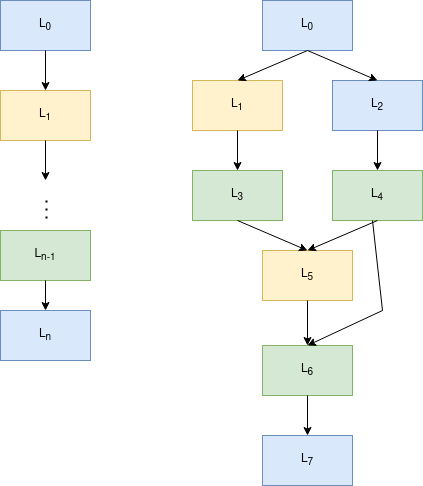
\includegraphics[scale=0.4]{space}
    \caption{Illustration of different ways to model neural architectures. Left: an example of a chain-structured NN.
             Right: an example of a multi-branch NN.}
    \label{space}
\end{figure}

% \begin{figure}
% \centering
%     \begin{subfigure}{0.1\textwidth}
%     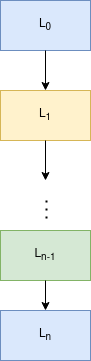
\includegraphics[width=\textwidth]{example}
%     \caption{First subfigure.}
%     \label{fig:first}
% \end{subfigure}
% \hfill
%     \begin{subfigure}{0.1\textwidth}
%     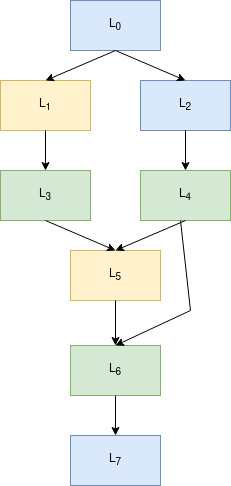
\includegraphics[width=\textwidth]{multi}
%     \caption{Second subfigure.}
%     \label{fig:second}
% \end{subfigure}
% \caption{Creating subfigures in \LaTeX.}
% \label{fig:figures}
% \end{figure}

\subsection{Search Strategy}
As any space search problem, there is a \textit{exploration-exploitation} trade-off to be considered \cite{elsken2019neural}.
Obtaining a high-performing architecture within a feasible amount of time is desired. However, converging too early to a
suboptimal result is also not the goal.

Based on the current state of the art, NAS search algorithms can be classified mainly intro three different
categories \cite{liu2021survey}:

\subsubsection{\textbf{Reinforcement Learning} (RL)-based NAS Algorithms}
Here, one considers the development of a neural architecture the agent's action, where the action space is the same as
the search space. Therefore, it is then possible to frame NAS as a reinforcement learning problem \cite{elsken2019neural}.
After evaluating the performance of the given trained architecture on fitness data, it is possible to
determine the agent's reward. How this estimation is performed will depend on the given method, more to these
approaches will be seen at \ref{PES}. Furthermore, how the agent's policy is represented and it's optimization will
also vary. More on trade-offs and details to these approaches will be seen in \ref{SOA}.

\subsubsection{\textbf{Gradient}-based NAS Algorithms}
\textcolor{black}{
Consists of transforming the search space from discrete to continuous and performing
gradient descent with respect to the fitness data set. This transformation requires a set of conditions
and has still not been mathematically proven \cite{liu2021survey}.
}

\subsubsection{\textbf{Evolutionary Computation} (EC)-based NAS Algorithms}
By the application of well established EC methods, which are various techniques based on the evolution of
species within nature, many different efforts were implemented to navigate their respective search space.
\textcolor{black}{
Among others, genetic algorithms (GAs), genetic programming (GP) and particle swarm optimization (PSO)
techniques have already been successfully applied.
}
More on these different techniques will be seen in \ref{EV}.

\subsection{Performance Estimation Strategy}
\label{PES}
Independent of the search strategy, it is necessary to know how any given architecture performed in order
to guide the next steps of the algorithm. There are many ways to estimate said performance, whereas the simplest
would be complete training and validation. Given the complexity and size of the search spaces within NAS, this
requires GPU days in the order of thousands \cite{elsken2019neural}. This is why extensive research has been
employed to reduce time on performance estimation, since it is a significant time bottleneck.
Some of these approaches include \cite{elsken2019neural}:
\begin{itemize}
    \item \textbf{Lower Fidelity Techniques}: Shorter training time \cite{zela2018towards}, \cite{zoph2018learning}, training solely on a
        subset of the data \cite{klein2018towards}, training on downscaled data \cite{chrabaszcz2017downsampled} or with downscaled
        models \cite{zoph2018learning}, \cite{pmlr-v70-real17a}. These methods do introduce bias as performances will normally be
        underestimated.

    \item \textbf{Learning Curve Extrapolation}: Performance is extrapolated after just a small number of epochs and then
        decided upon directly. Klein et al. \cite{klein2018towards} considered architectural hyperparameters to predict which
        architectures are most promising after partial learning. Domhan et al \cite{domhan2015speeding} extrapolated partial
        learning curves to predict and eliminate sub-optimal architectures.

    \item \textbf{Weight Inheritance}: also dubbed as \textit{network morphisms} is a technique that passes down weights from
        previously trained models forward to new ones. This approach can cut down computational costs to just a few GPU days
        \cite{cai2018efficient}.

    \item \textbf{One-Shot Models}: also called \textit{weight sharing} is a technique that treats all architectures as subgraphs
        of a supergraph, which is named the one-shot model. Weights are shared between architectures that meet the condition of
        having edges in common. Finally, only the weights of a single one-shot model has to be trained and the
        sub-graph architectures can be evaluated directly as they inherit weights from the one-shot model. This demonstrates great
        success by cutting-down the entire process to a few GPU days. However, significant bias is introduced as the underestimation of architectures by this approach is harsh.
\end{itemize}

\section{State of the Art}
\label{SOA}

\subsection{Overview}
Currently RL-based algorithms are extremely costly in terms of computation, requiring thousands of
graphics processing cards (GPUs) for days. This is already the case for median-scale data sets, as
as data grows more complex, so does the processing time needed to search for a suitable architecture.

Gradient-based algorithms are faster, there are examples such as the DARTS algorithm, where processing power
is cut down to single digit GPUs \cite{liu2018darts}. However, due to the not completely compatible relationship
of NAS and a gradient-based optimization, frequently sub-optimal architectures are found \cite{liu2021survey}.

On the other hand, EC methods, while not perfect, have been around for decades and are easily applicable
to solve complex non-convex optimization problems, as they are insensitive to local minima and do not require
gradient information \cite{liu2021survey}.

\subsection{Evolutionary Neural Architecture Search (ENAS)}
\label{EV}

\begin{figure}[!h]
    \centering
    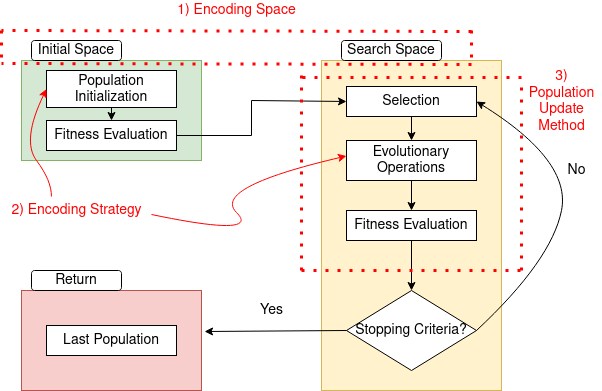
\includegraphics[scale=0.4]{evol}
    \caption{Generic flowchart of a typical ENAS algorithm}
    \label{evol}
\end{figure}

ENAS algorithms are NAS algorithms that leverage existing evolutionary computational methods
to search for an optimal architecture within a defined search space.

Any ENAS algorithm can be broken down into a series of steps exemplified by Fig. \ref{evol}. The term \textit{population} seen
in Fig. \ref{evol} is defined as a
a finite number of \textit{individuals}, where each individual is any given neural architecture or model within the defined  search space.

At the beginning of the algorithm an initial population is created within a pre-defined initial space.
Then, their fitness is evaluated, which essentially is the process of performance estimation already covered in \ref{PES}
for each individual in this generation's population. Finally, this population undergoes a repetitive process that
includes \textit{selection}, \textit{evolutionary operations} and once again a fitness evaluation. If the resulting
population meet the defined goal, the final architecture has been found. Otherwise repeat the last process until this
goal is reached.

Having understood the main steps of an ENAS implementation, it becomes clear that ENAS methods can be
differentiated by their \cite{liu2021survey}:
\begin{itemize}
    \item \textbf{Encoding Space}: contains all valid individuals (architectures) within a given population.

    \item \textbf{Encoding Strategy}: How architectures are represented within the encoding space.

    \item \textbf{Population Update Method}: These are the selection strategies, how the evolutionary operators are applied
        and how populations are ultimately updated.

    \item \textbf{Fitness Evaluation}: The same concept of performance estimation strategy already touched on
        in \ref{PES}.
\end{itemize}

In the following subsections, state of the art ENAS methods will be discussed and illustrated through
the lense of these different elements that compose an ENAS algorithm. Although, ENAS encompasses many different
techniques such as evolutionary algorithms (EA), Swarm Intelligence (SI) methods and many others;
this work will focus mostly on EA, since the vast majority of relevant ENAS research have utilized it.

\subsubsection{Encoding Space}
The encoding space can be further divided into the initial space and the search space. These two may be the same in some cases,
but often are not. The initial space is the set of all possible architectures that any individual in the initial population may
become. There are three types of architecture initialization approaches \cite{liu2021survey}: starting from trivial conditions,
rich initialization and random initialization in the encoding space.

The trivial space approach has been done by \cite{pmlr-v70-real17a}
and had the benefit of giving much more freedom to the algorithm to explore unseen architectures and also justifies well
the used of EC-methods instead of any other. However, this comes at the cost of high computational resources.

The rich initialization method, also named \textit{well-designed space}, consists of initializing the population within
a set of state-of-the-art architectures. This way, a good architecture can be found early on and potentially decrease
search time. On the other hand, finding novel architectures is very improbable.

\subsubsection{Encoding Strategy} (TBD)
\subsubsection{Population Update}
Genetic Algorithm (GA)-based ENAS is the most popular approach among ENAS methods, since architecture representation is
very convenient in GA \cite{liu2021survey}. The selection is the first stage of updating the current population and can
be divided into several strategies, four of whom are widely used: Elitism, Discard worst or oldest, Roulette and Tournament
Selection.

Works such as \cite{elsken2017simple} take use of elitism, where essentially only the fittest of individuals are selected to
compose the next population. This can cause a loss of diversity, as there is a chance that similar architectures perform
similarly well and thus may cause generations to breed only akin individuals, since only the fittest are kept. This in turn,
can cause the population to fall within a local optima and not being able to explore efficiently.

Other approaches such as \cite{pmlr-v70-real17a} and \cite{zhang2019identify} discarded the oldest individual from the population,
which is also known as aging evolution. This ensures that the search does not focus on good models too early and therefore
performs a more broad search of the encoding space in comparison to non-aging evolution.

There is also the possibility to combine different strategies such as in \cite{zhu2019eena}, where both discarding the worst and the oldest
were used.

\subsection{NAS and tinyML}
Machine learning on small microcontrollers is a great ambition. TinyML is the field that answers to that challenge
and aims to provide intelligent features to even a \$5 device, such as an off-the-shelf microcontroller. This is not a
small effort as microcontrollers possess very limited resources, especially concerning memory and storage. In the following
subsections, relevant work that combined NAS algorithms within the tinyML universe will be shown.

\subsubsection{\textbf{MCUNet}}

MCUNet, a framework that shows promising results, is composed of
two major components: the efficient neural architecture (TinyNAS) and the lightweight inference engine (TinyEngine) \cite{lin2020mcunet}.
The TinyNAS algorithm is a two-stage neural architecture search method, where firstly it optimizes the search space according to the
given resource constraints and then performs an ENAS algorithm to find the best architecture within this new search space.
Since the performance of NAS methods depend strongly on the search space \cite{radosavovic2020designing}, this technique
through extra constaints forces the search to consider a smaller set, where only architectures that fit the desired requirements
can be found. These requirements may be limited memory consumption, storage limits, latency and even energy.

MCUNet used weight sharing \cite{lin2020mcunet}, where a single super network is created, which contains all the
sub-networks in the search space. This method leverages the graph attribute of these networks to share weights among
subnetworks and drastically reduce the time needed to train all possible individuals.

The ENAS algorithm used in MCUNet uses elitism as its selection strategy, always choosing the top-20 individuals in
terms of accuracy within a given generation. Crossover is applied to generate 50 new candidates and then mutation with a
probablity of 10\% is used to generate the remaining 50. All generations are of size 100. Finally, after 30 iterations,
the fittest architecture is chosen.

In addition to that, TinyEngine implements a code generator-based compilation method that not only eliminates memory overhead, but also improves
the speed of inference as well \cite{lin2020mcunet}. This addresses the shortcomings of similar libraries such as TF-Lite
Micro \cite{abadi2016tensorflow} and CMSIS-NN \cite{lai1801efficient} that opt for runtime interpretation of code instead.

Finally, this work has shown to be able to reduce memory usage by 2.7x and improve inference speed by 1.7-2.2
compared to TF-Lite Micro and CMSIS-NN, also decreased code size by up to 4.5X and 5.0x for TF-Lite Micro and CMSIS-NN
respectively \cite{lin2020mcunet}. MCUnet achieved state of the art performance, taking 12.5 GPU days to design a model
\cite{lin2020mcunet}. This is a great improvement compared to MnasNET, which took 40,000 GPU hours for the same
data set \cite{tan2019mnasnet} and is also faster than most NAS methods performed on regular machines.

\section{Conclusion}
Throughout this work a brief overview of the current research on NAS has been displayed. NAS is not only
a complex optimization problem, but also one that requires significant computational resources in most applications. The
trade-offs of the mainstream approaches to NAS have also been demonstrated, whilst also highlighting efforts done with the
use of EC-based approaches.

In addition to that, different applications of NAS methods within the tinyML paradigm have been illustrated.
For IoT devices and microcontrollers it is not only needed to train models considering performance,
but also considering other parameters such as latency, memory usage and even energy preservation.

% references section
\newpage
\bibliographystyle{IEEEtran}
\bibliography{refs}

%
\end{document}
